%%%%%%%%%%%%
%
% $Autor: Sandesh Nonavinakere Sunil $
% $Datum: today $
% $Pfad: PythonPackages/Contents/General/LineaPy $
% $Version: 4250 $
% !TeX spellcheck = en_GB/de_DE
% !TeX encoding = utf8
% !TeX root = filename
% !TeX TXS-program:bibliography = txs:///biber
%
%%%%%%%%%%%%
	
	\chapter{Package \texttt{LineaPy}}
	
	\section{Introduction} 
		LineaPy is a Python package designed to capture, analyze, and automate data science workflows. By tracing the sequence of code execution, LineaPy provides tools that assist data scientists in transitioning their work from development to production efficiently, often with just two lines of code \cite{lineapy_docs}.
	\section{Description}
		In data science, moving from prototype to production can be challenging due to the manual and time-consuming engineering processes required to clean and structure code. LineaPy addresses this by capturing the sequence of code execution, enabling the automatic transformation of exploratory code into production-ready pipelines. This capability reduces friction in the development process and accelerates deployment \cite{lineapy_github}.
		
		\begin{figure}[h!]
			\centering
			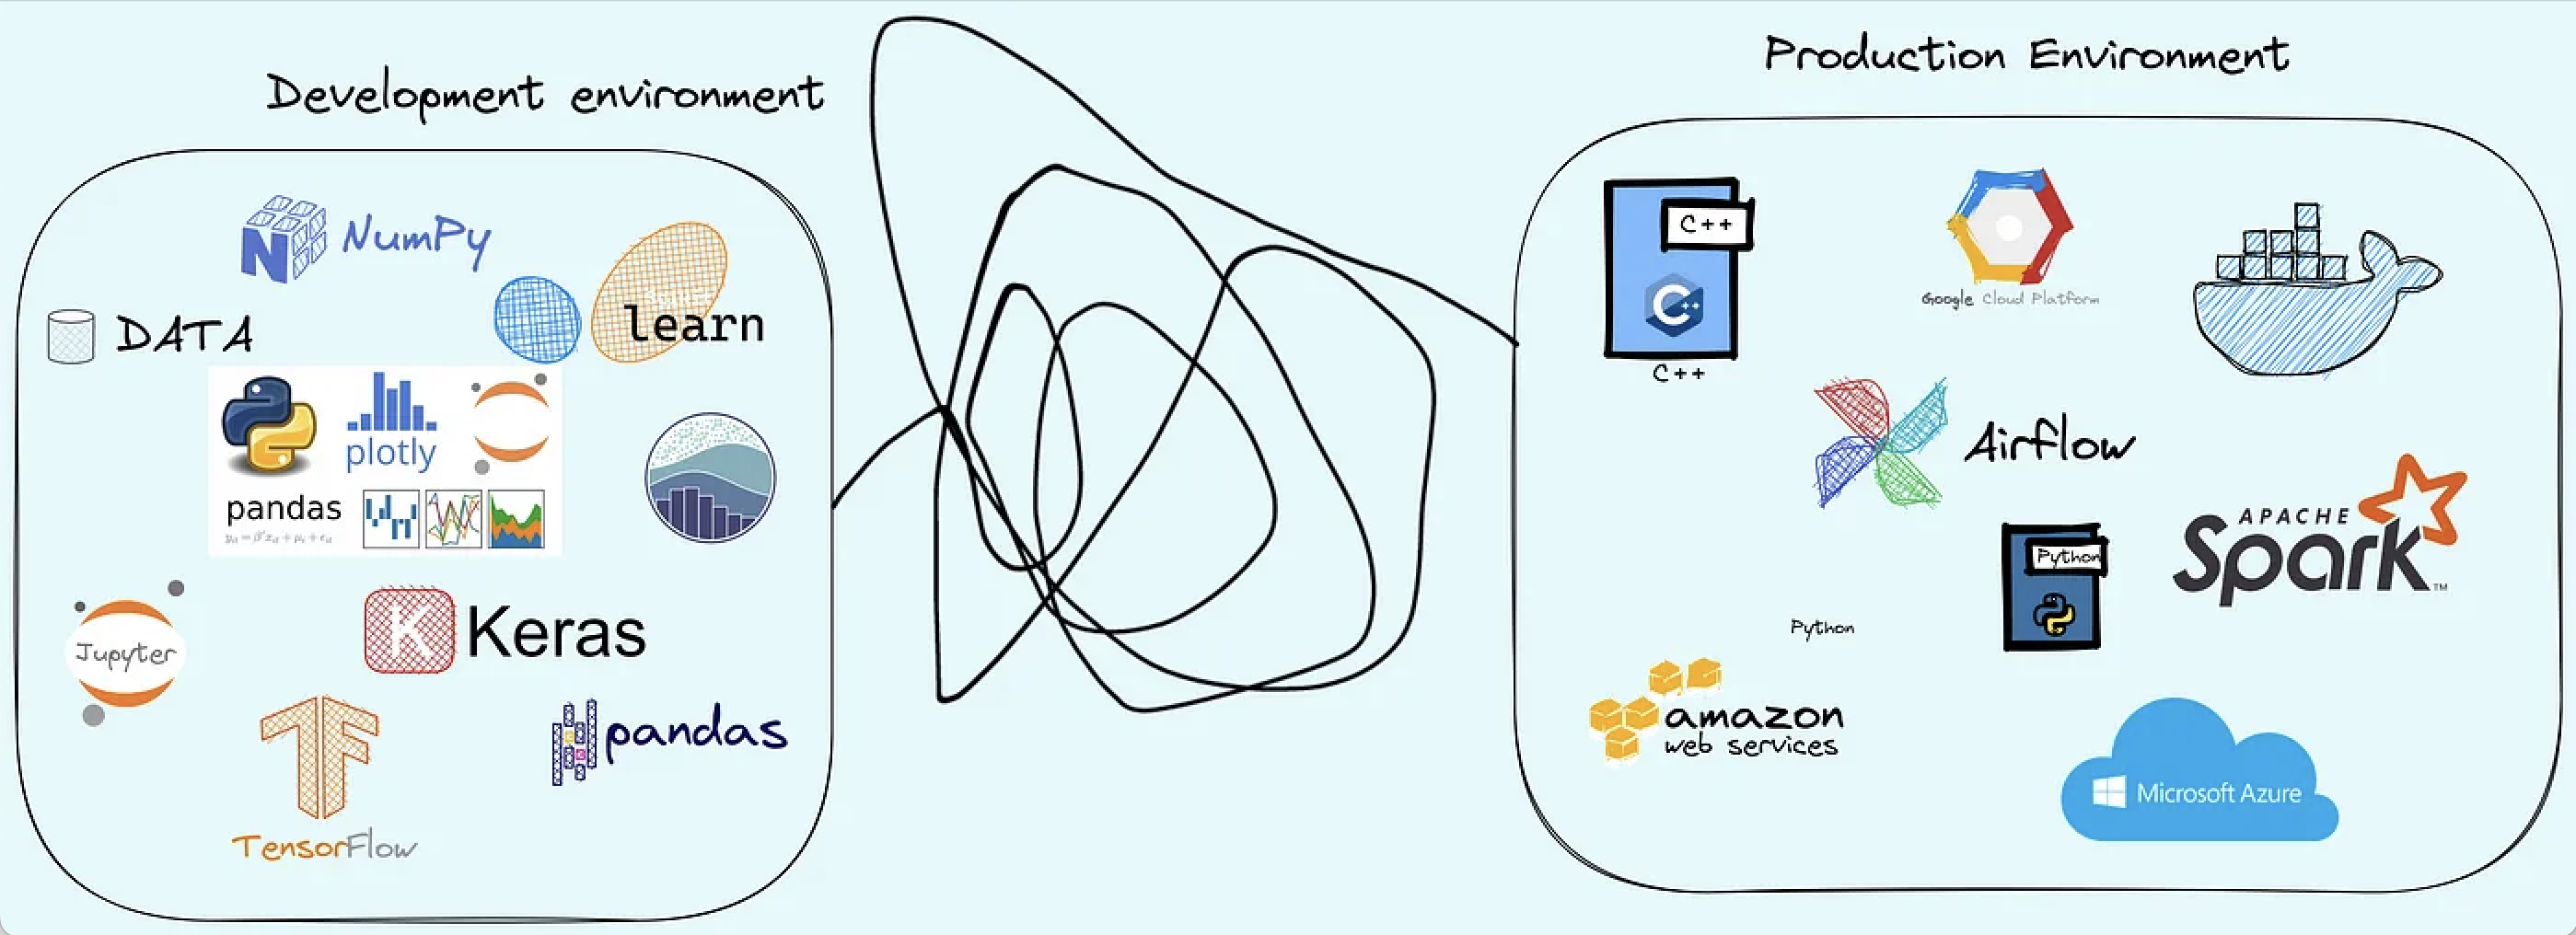
\includegraphics[scale=0.25]{Lineapy/Lineapyintro.png}
			\caption{Lineapyintro}
			\label{fig:Lineapyintro}
		\end{figure}
		
	\section{Installation}
	To install LineaPy, ensure that your environment meets the following prerequisites:
	\begin{itemize}
		\item Python version: \texttt{>=3.7,<3.11}
		\item IPython version: \texttt{>=7.0.0}
	\end{itemize}
	You can install LineaPy using pip:
	\begin{lstlisting}
		pip install lineapy
	\end{lstlisting}
	For additional installation options, such as support for PostgreSQL or Amazon S3, refer to the official documentation \cite{lineapy_github}.
	\section{Example}
		This section provides a comprehensive example demonstrating how to use LineaPy in a typical data science workflow.
	
	\subsection{Description}
	Consider a scenario where you have developed a data analysis script in a Jupyter notebook. The code involves data loading, preprocessing, model training, and evaluation. Using LineaPy, you can capture this workflow and transform it into a production-ready pipeline with minimal effort.
	\subsection{Manual}
		1. Import LineaPy: Begin by importing the LineaPy package into your Python environment.
	2. Capture Artifacts: Identify key variables or outputs in your code that you wish to capture as artifacts.
	3. Save Artifacts: Use LineaPy's API to save these artifacts, specifying names and descriptions.
	4. Generate Pipeline: Instruct LineaPy to generate a pipeline script based on the captured artifacts and their dependencies.
	\subsection{Code}
	
	
	
	\begin{lstlisting}
		import lineapy
		
		# Data loading
		data = load_data('data.csv')
		
		# Data preprocessing
		clean_data = preprocess(data)
		
		# Model training
		model = train_model(clean_data)
		
		# Save the trained model as an artifact
		lineapy.save(model, 'trained_model')
		
		# Generate a pipeline script
		lineapy.to_pipeline('trained_model', 'pipeline_script.py')
	\end{lstlisting}
	\subsection{Files}
The typical outputs from LineaPy when it is used to automate workflow management and pipeline generation are listed below. Here's what each file represents and how it fits into the generated system:

 \begin{enumerate}
 	\item \textbf{module.py} \linebreak
 	\textbf{Description: }
 	\begin{itemize}
 		\item This file contains the core Python code for the pipeline. It is typically a modularized version of your script, where reusable functions, classes, or objects are refactored into a module.
 	    \item Includes all logic and computations, including data processing, machine learning, or any other transformations.
 		\end{itemize}
 		
 	\textbf{Usage:} 
 	\begin{itemize}
 		\item Can be imported into other scripts or workflows.
 	    \item Acts as a central reference for executing pipeline tasks.
 \end{itemize}
 
 	\item \textbf{requirements.txt} \linebreak
 	\textbf{Description:} 
 	\begin{itemize}
 		\item A list of all Python dependencies required to execute the pipeline, such as libraries for data processing (e.g., `pandas`, `numpy`), machine learning (e.g., `scikit-learn`), or workflow orchestration.
 \end{itemize}
 	\textbf{Usage:}
 	\begin{itemize}
 		\item Ensures all necessary packages are installed before running the pipeline.
 	   \item Typically used with the below code to set up the environment.
 		\end{itemize}
 		
 	\begin{lstlisting}
 		pip install -r my_pipeline_requirements.txt
 	\end{lstlisting} 
 	
 	\item \textbf{params.yaml} \linebreak
 \textbf{	Description: }
 \begin{itemize} 
 	  \item Contains configuration parameters for the pipeline, such as file paths, data source locations, model hyperparameters, or execution flags.
 	\item Acts as a central place to modify pipeline configurations without changing the core logic.
 	
 \textbf{	Usage:}
 	\item Allows for flexibility and reusability of the pipeline across different datasets or environments.
 	\item Read dynamically by pipeline scripts to adjust behavior.
 \end{itemize}
 
 	\item \textbf{task1.py and task1.py} \linebreak
 	\textbf{Description:}
 	\begin{itemize}
 		\item These are individual task scripts representing specific steps in the pipeline. For example:
 	\item task1.py: Might handle data preprocessing.
 	\item task2.py: Could handle model training or evaluation.
 	\item They often include the isolated logic needed to execute a single part of the workflow.
 	
 	\textbf{Usage:}
 	\item Used in a task-based workflow, where each file is executed as part of a sequence defined by a Directed Acyclic Graph (DAG).
 	\item Helps with modular execution and debugging.
 		\end{itemize}
 		
 	\item  \textbf{dvc.yaml} \linebreak
 	\textbf{Description:}
 	\begin{itemize}
 		\item A configuration file for Data Version Control (DVC), which is used to track changes in data, models, and pipeline workflows.
 	\item It defines the stages of your pipeline, the dependencies for each stage, and the outputs produced.
 	
 	\textbf{Usage:}
 	\item Ensures reproducibility by tracking data and model changes across different runs.
 	\item Used with `dvc repro` to execute the pipeline and verify dependencies.
 \end{itemize}
 
 	\item \textbf{Dockerfile} \linebreak
 	\textbf{Description:}
 	\begin{itemize}
 		\item A Dockerfile for containerizing the entire pipeline. It specifies the environment, dependencies, and runtime setup required to execute the workflow.
 	\item Includes commands like `COPY`, `RUN`, and `CMD` to configure a Docker image.
 	
 	\textbf{Usage:}
 	\item Allows the pipeline to run consistently across different environments.
 	\item Used to build a Docker image .
 \end{itemize}
 \end{enumerate}

\textbf{ How These Files Work Together}
\begin{enumerate}
	\item Code: 
	`module.py` (core logic) and `task1.py` / `task2.py` (individual steps).
	\item Environment: 
	- `requirements.txt` (Python dependencies) and `Dockerfile` (containerization).
	\item Configuration: 
	- `params.yaml` and `dvc.yaml` (workflow definitions and versioning).
	\item Execution: 
	- The orchestrator (e.g., DVC or Airflow) uses these files to execute tasks in the correct sequence, ensuring reproducibility and modularity.
\end{enumerate}

\begin{figure}[h!]
	\centering
	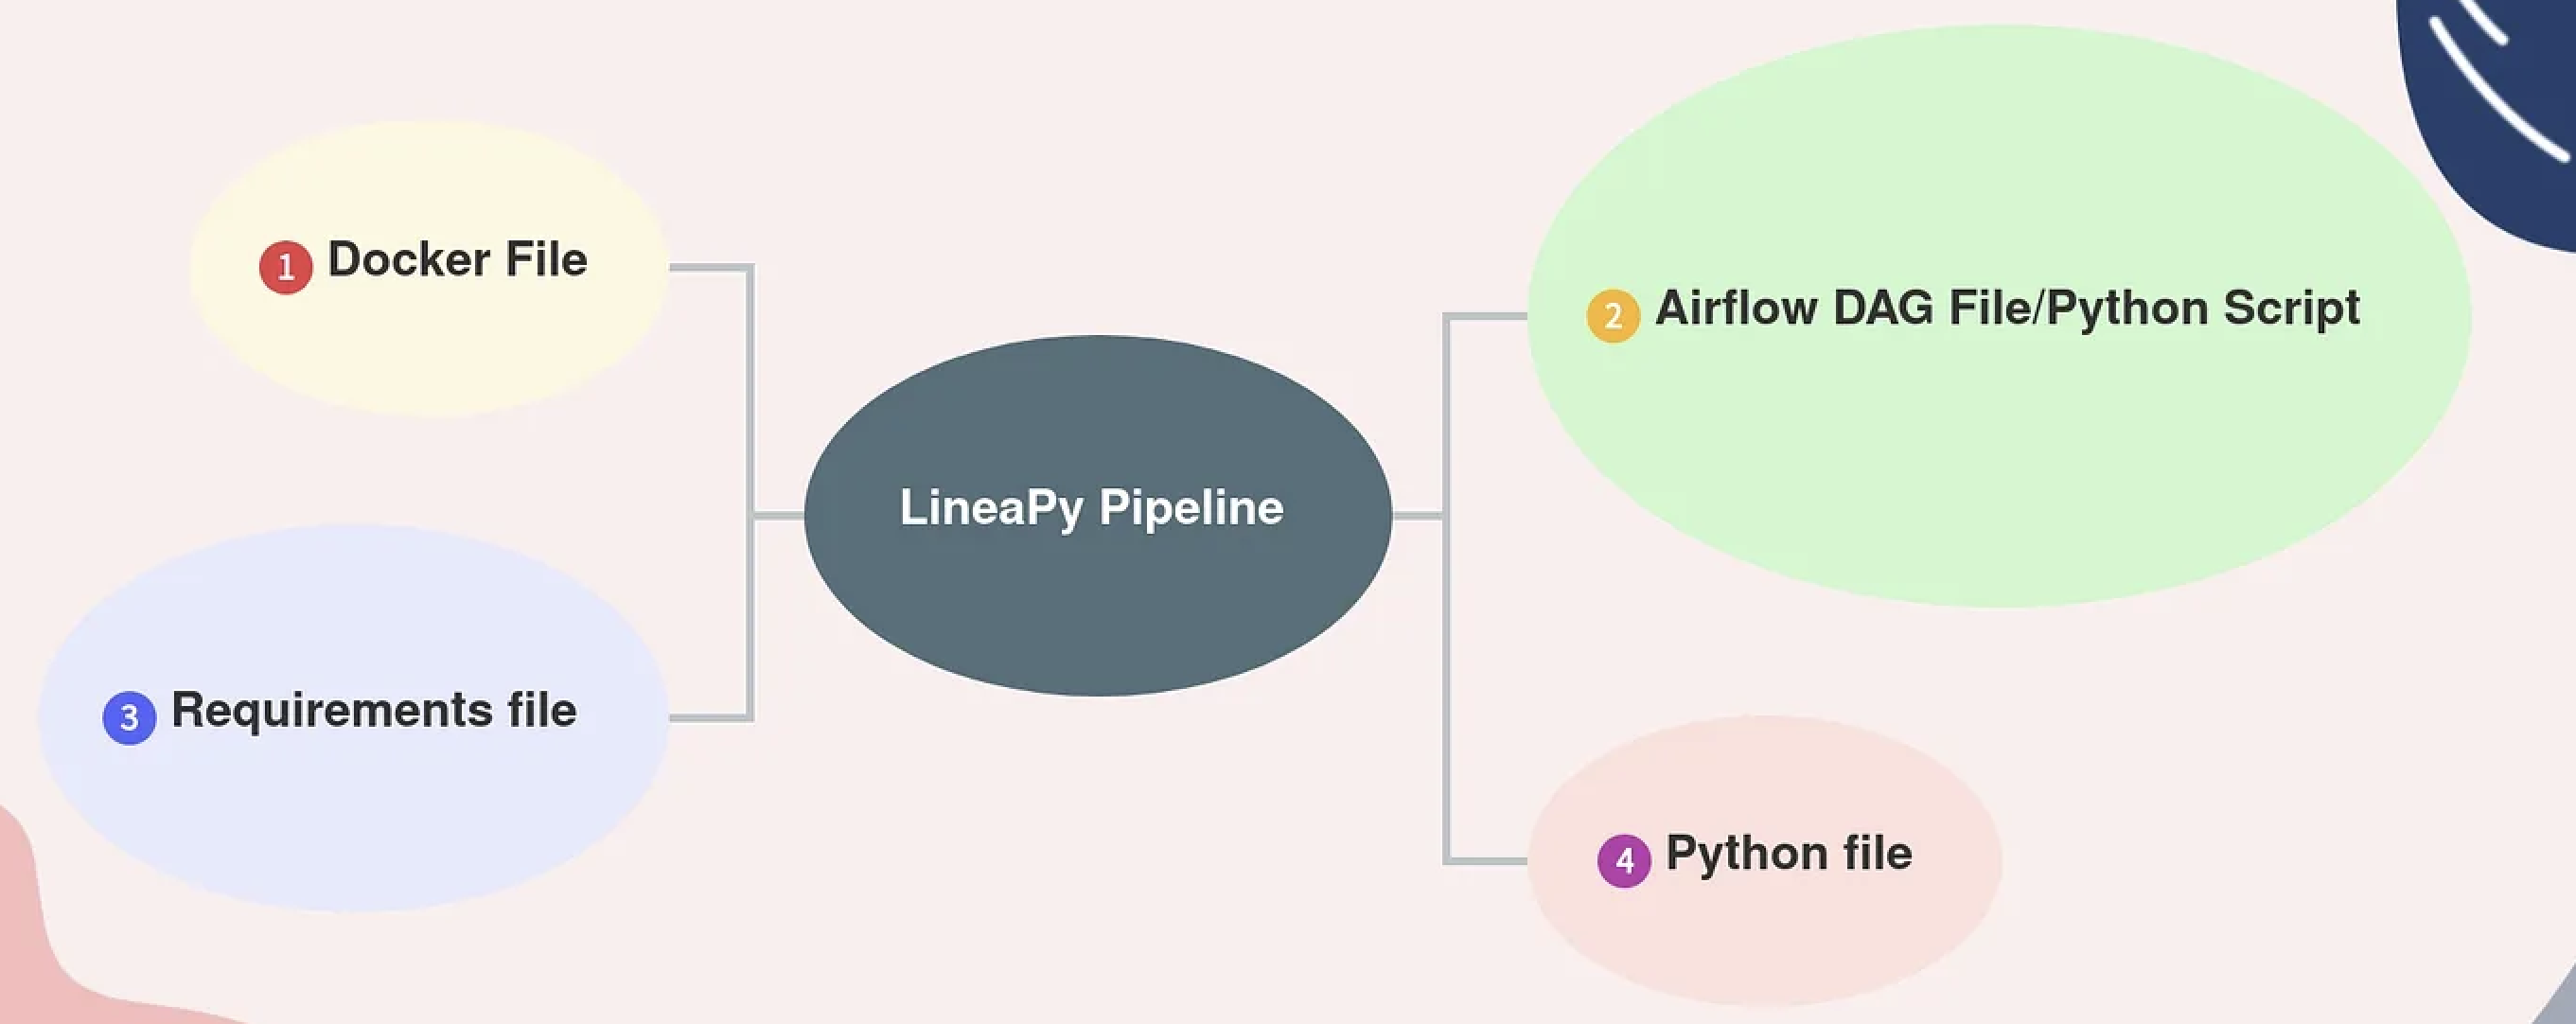
\includegraphics[scale=0.3]{Lineapy/FilegenerationLineapy.png}
	\caption{Main types of file outputs of Lineapy}
	\label{fig:Main types of file outputs of Lineapy}
\end{figure}

\pagebreak
	
		\subsection{Detailed walkthrough Example}

About the dataset: The dataset is the Auto MPG dataset available at
\href{https://archive.ics.uci.edu/ml/datasets/auto+mpg}{UCI Machine learning Repository} Center for Machine Learning and Intelligent Systems.

The below example is a classic regression problem.Use the classic Auto MPG dataset and demonstrate how to build models to predict the fuel efficiency of the late-1970s and early 1980s automobiles. To do this, you will provide the models with a description of many automobiles from that time period. This description includes attributes like cylinders, displacement, horsepower, and weight.

This is the high level workflow in which the code runs.
\begin{enumerate}
	\item Load the train and test data into a pandas dataframe
	\item EDA and Statistical Analysis.
	\item Save the final training and test data as an artifact-Use save()
	\item Check the artifact-get()
	\item Build the model using different methods.
	\item Choose the best model.
	\item Save the best model as an artifact-save()
	\item Display the artifact catalog-catalog()
	\item Build the pipeline using the saved artifacts.
\end{enumerate}
	
	\pagebreak
	
	\textbf{Declare all the necessary packages.}
	\begin{lstlisting}[language=Python]
		%%capture
		import IPython
		
		/**
		* Check the version of IPython installed.
		* If the version is lower than 7, upgrade it.
		*/
		if (IPython.version_info[0] < 7):
		!pip -q install ipython --upgrade
		/**
		* Exit the runtime to apply the updated version of IPython.
		*/
		exit()
		/**
		* The following cell will execute after the runtime restart.
		*/
		
		# Use seaborn for pairplot.
		!pip install -q seaborn
		
		%%capture
		!pip -q install lineapy
		
		%load_ext lineapy
		
		import os
		import lineapy
		
		import matplotlib.pyplot as plt
		import numpy as np
		import pandas as pd
		import seaborn as sns
		
		/**
		* Set NumPy print options to improve readability of the output.
		*/
		np.set_printoptions(precision=3, suppress=True)
		
		import tensorflow as tf
		
		from tensorflow import keras
		from tensorflow.keras import layers
		
		/**
		* Print the TensorFlow version to verify the correct installation.
		*/
		print(tf.__version__)
	\end{lstlisting}
	
	\pagebreak
	\textbf{Download the dataset and upload the data into a pandas dataframe.}
\begin{lstlisting}[language=Python]
	/**
	* @file auto_mpg_data_loader.py
	* @brief This script loads the Auto MPG dataset from the UCI Machine Learning Repository
	*        and prepares it for analysis.
	* 
	* @details This script reads the dataset from the given URL, assigns column names to the
	*          dataset, handles missing values represented by `?`, and prepares the dataset
	*          for further processing.
	* 
	* @version 1.0
	* @date 2025-01-24
	*/
	
	/**
	* @brief URL of the Auto MPG dataset.
	* 
	* This URL points to the location of the Auto MPG dataset on the UCI Machine Learning
	* Repository.
	* 
	* @see https://archive.ics.uci.edu/ml/machine-learning-databases/auto-mpg/
	*/
	url = 'http://archive.ics.uci.edu/ml/machine-learning-databases/auto-mpg/auto-mpg.data'
	
	/**
	* @brief List of column names for the Auto MPG dataset.
	* 
	* These column names correspond to various attributes in the dataset such as MPG,
	* Cylinders, Displacement, Horsepower, etc.
	*/
	column_names = ['MPG', 'Cylinders', 'Displacement', 'Horsepower', 'Weight',
	'Acceleration', 'Model Year', 'Origin']
	
	/**
	* @brief Reads and loads the Auto MPG dataset from the specified URL.
	* 
	* This function uses `pandas.read_csv()` to read the dataset, assign appropriate column
	* names, handle missing values marked by `?`, and skips initial whitespace.
	* 
	* @note The dataset is separated by spaces and tabs. Missing values are represented as `?`.
	* 
	* @param url The URL from which the dataset will be loaded.
	* @param column_names List of column names to assign to the dataset.
	* 
	* @return A pandas DataFrame containing the loaded Auto MPG dataset.
	*/
	raw_dataset = pd.read_csv(url, names=column_names,
	na_values='?', comment='\t',
	sep=' ', skipinitialspace=True)
\end{lstlisting}
	
	\pagebreak
	\textbf{Now do some exploratory data analysis and statistical analysis.}
	\begin{lstlisting}[language=Python]
		# dataset = raw_dataset.copy()
		# dataset.tail()
		#
		# @brief This part of the code is used to create a copy of the raw dataset and display the last few rows.
		dataset = raw_dataset.copy()
		dataset.tail()
		
		# dataset.isna().sum()
		# @brief This command counts the number of missing (NA) values in each column of the dataset.
		dataset.isna().sum()
		
		# #drop na
		# @brief Drops all rows with missing values from the dataset.
		dataset = dataset.dropna()
		
		# dataset['Origin'] = dataset['Origin'].map({1: 'USA', 2: 'Europe', 3: 'Japan'})
		# @brief Maps numerical values in the 'Origin' column to their respective string categories.
		dataset['Origin'] = dataset['Origin'].map({1: 'USA', 2: 'Europe', 3: 'Japan'})
		
		# #one hot encoding
		# @brief Performs one-hot encoding on the 'Origin' column and drops the prefix.
		dataset = pd.get_dummies(dataset, columns=['Origin'], prefix='', prefix_sep='')
		
		# dataset.tail()
		# @brief Displays the last few rows of the dataset after one-hot encoding.
		dataset.tail()
		
		# train_dataset = dataset.sample(frac=0.8, random_state=0)
		# @brief Splits the dataset into training and testing datasets, with 80% for training.
		train_dataset = dataset.sample(frac=0.8, random_state=0)
		
		# test_dataset = dataset.drop(train_dataset.index)
		# @brief Creates the testing dataset by dropping the training rows.
		test_dataset = dataset.drop(train_dataset.index)
		
		# sns.pairplot(train_dataset[['MPG', 'Cylinders', 'Displacement', 'Weight']], diag_kind='kde')
		# @brief Generates a pairplot of selected features ('MPG', 'Cylinders', 'Displacement', 'Weight') for visual exploration.
		sns.pairplot(train_dataset[['MPG', 'Cylinders', 'Displacement', 'Weight']], diag_kind='kde')
		
		# train_dataset.describe().transpose()
		# @brief Describes the training dataset with statistics (mean, std, etc.) and transposes the output for easier readability.
		train_dataset.describe().transpose()
		
		# #normalization
		# @brief This block performs normalization by first displaying the mean and std of the dataset, 
		# then applying a TensorFlow normalizer to scale the features.
		train_dataset.describe().transpose()[['mean', 'std']]
		
		normalizer = tf.keras.layers.Normalization(axis=-1)
		normalizer.adapt(np.array(train_features))
		
		# print(normalizer.mean.numpy())
		# @brief Displays the calculated mean of the training features after normalization.
		print(normalizer.mean.numpy())
		
		# first = np.array(train_features[:1])
		# @brief Extracts the first row from the training features to examine how it is normalized.
		first = np.array(train_features[:1])
		
		# with np.printoptions(precision=2, suppress=True):
		# @brief Displays the first example and its normalized form with a specified precision.
		with np.printoptions(precision=2, suppress=True):
		print('First example:', first)
		print()
		print('Normalized:', normalizer(first).numpy())
	\end{lstlisting}
	
	\pagebreak
	\textbf{Now save the train and test data dataframes as artifacts-save()}
	
	\begin{lstlisting}[language=Python]
		# Store the variable as an artifact
		# @brief Save the train_features as an artifact using lineapy.save() and store the result in train_artifact
		train_artifact = lineapy.save(train_features, "train_data")
		
		# @brief Check the type of the object stored in train_artifact
		# @details This prints the type of train_artifact to help understand its data structure.
		print(type(train_artifact))
		
		# Store the variable as an artifact
		# @brief Save the train_labels as an artifact using lineapy.save() and store the result in train_labels
		train_labels = lineapy.save(train_labels, "train_labels")
		
		# @brief Check the type of the object stored in train_labels
		# @details This prints the type of train_labels to help understand its data structure.
		print(type(train_labels))
		
		# Store the variable as an artifact
		# @brief Save the test_features as an artifact using lineapy.save() and store the result in test_artifact
		test_artifact = lineapy.save(test_features, "test_data")
		
		# @brief Check the type of the object stored in test_artifact
		# @details This prints the type of test_artifact to help understand its data structure.
		print(type(test_artifact))
		
		# Store the variable as an artifact
		# @brief Save the test_labels as an artifact using lineapy.save() and store the result in test_labels
		test_labels = lineapy.save(test_labels, "test_labels")
		
		# @brief Check the type of the object stored in test_labels
		# @details This prints the type of test_labels to help understand its data structure.
		print(type(test_labels))
	\end{lstlisting}
	
	\pagebreak
	Now build the models and choose the best model. You can use the artifacts stored previously to get the pre-processed train and test data sets.
	
	\textbf{1st model: Linear Regression Model}
	
	\begin{lstlisting}[language=Python]
		/**
		* @file linear_regression_model.py
		* @brief This script builds, trains, and evaluates a simple linear regression model using TensorFlow.
		*/
		
		# Import necessary libraries (assumed)
		import tensorflow as tf
		from tensorflow.keras import layers
		
		/**
		* @brief Sequential model for linear regression.
		* @details The model consists of a normalizer layer and a dense layer with one unit (output).
		*/
		linear_model = tf.keras.Sequential([
		normalizer, /**< Data normalizer layer */
		layers.Dense(units=1) /**< Dense layer with one output unit for regression */
		])
		
		/**
		* @brief Make predictions using the trained linear model.
		* @param train_features1 The input features for prediction.
		* @return Predictions for the first 10 samples in the training dataset.
		*/
		linear_model.predict(train_features1[:10])
		
		/**
		* @brief Retrieve the kernel weights of the Dense layer (first layer in the model).
		* @return The kernel weights of the first dense layer.
		*/
		linear_model.layers[1].kernel
		
		/**
		* @brief Compile the linear regression model.
		* @param optimizer The optimizer used for training (Adam with learning rate 0.1).
		* @param loss The loss function used to evaluate the model (mean absolute error).
		*/
		linear_model.compile(
		optimizer=tf.optimizers.Adam(learning_rate=0.1), /**< Optimizer with learning rate 0.1 */
		loss='mean_absolute_error' /**< Loss function to minimize */
		)
		
		/**
		* @brief Train the linear model.
		* @param train_features1 The input features for training.
		* @param train_labels1 The target labels for training.
		* @param epochs Number of epochs for training.
		* @param validation_split Fraction of training data to use for validation.
		* @return History object containing training details.
		*/
		history = linear_model.fit(
		train_features1, /**< Features for model training */
		train_labels1, /**< Labels for model training */
		epochs=100, /**< Number of training epochs */
		verbose=0, /**< Suppress logging during training */
		validation_split=0.2 /**< Use 20% of training data for validation */
		)
		
		/**
		* @brief Plot the loss over epochs.
		* @param history The history object returned by model.fit().
		*/
		def plot_loss(history):
		plt.plot(history.history['loss'], label='loss') /**< Plot training loss */
		plt.plot(history.history['val_loss'], label='val_loss') /**< Plot validation loss */
		plt.ylim([0, 10]) /**< Set y-axis range for better visibility */
		plt.xlabel('Epoch') /**< Label for x-axis */
		plt.ylabel('Error [MPG]') /**< Label for y-axis */
		plt.legend() /**< Show legend */
		plt.grid(True) /**< Show grid for better readability */
		
		/**
		* @brief Generate a plot of the loss curves.
		* @param history The history object containing training details.
		*/
		plot_loss(history)
		
		# Evaluate the model on the test dataset
		/**
		* @brief Evaluate the trained model on the test data.
		* @return A dictionary containing the evaluation result for the linear model.
		*/
		test_results = {}
		test_results['linear_model'] = linear_model.evaluate(
		test_features1, test_labels1, verbose=0) /**< Evaluate on test data */
	\end{lstlisting}
	
	\pagebreak
	\textbf{2nd Model-DNN Model:}
	
	\begin{lstlisting}[language=Python]
	## \file dnn_model.py
	#  \brief This script builds, compiles, trains, and evaluates a Deep Neural Network (DNN) model.
	
	import tensorflow as tf
	from tensorflow import keras
	from tensorflow.keras import layers
	import matplotlib.pyplot as plt
	
	## \brief Builds and compiles a DNN model.
	#  \param norm Normalization layer to preprocess input features.
	#  \return A compiled Keras Sequential model.
	def build_and_compile_model(norm):
	model = keras.Sequential([
	norm,
	layers.Dense(64, activation='relu'),  # First hidden layer with 64 neurons and ReLU activation.
	layers.Dense(64, activation='relu'),  # Second hidden layer with 64 neurons and ReLU activation.
	layers.Dense(1)  # Output layer with 1 neuron (for regression tasks).
	])
	
	# Compile the model with mean absolute error loss and Adam optimizer.
	model.compile(
	loss='mean_absolute_error',
	optimizer=tf.keras.optimizers.Adam(0.001)
	)
	return model
	
	# Build and compile the model using the provided normalizer.
	## \var dnn_model
	#  \brief Instance of the compiled DNN model.
	dnn_model = build_and_compile_model(normalizer)
	
	# Display the model architecture.
	dnn_model.summary()
	
	## \brief Train the DNN model on the training dataset.
	#  \param train_features1 Training features used as input for the model.
	#  \param train_labels1 Ground truth labels corresponding to training features.
	#  \param validation_split Fraction of data to use for validation.
	#  \param epochs Number of training epochs.
	#  \return Training history object containing loss and validation loss.
	history = dnn_model.fit(
	train_features1,  # Input features for training.
	train_labels1,    # Ground truth labels.
	validation_split=0.2,  # Use 20% of data for validation.
	verbose=0,  # Suppress detailed logging.
	epochs=100  # Train for 100 epochs.
	)
	
	## \brief Plots training and validation loss over epochs.
	#  \param history Training history object containing loss and validation loss.
	def plot_loss(history):
	plt.plot(history.history['loss'], label='loss')  # Plot training loss.
	plt.plot(history.history['val_loss'], label='val_loss')  # Plot validation loss.
	plt.ylim([0, 10])  # Set Y-axis limits.
	plt.xlabel('Epoch')  # Label for the X-axis.
	plt.ylabel('Error [MPG]')  # Label for the Y-axis.
	plt.legend()  # Add legend to the plot.
	plt.grid(True)  # Add grid lines to the plot.
	plt.show()  # Display the plot.
	
	# Call the function to plot loss.
	plot_loss(history)
	
	## \brief Evaluate the trained DNN model on the test dataset.
	#  \param test_features1 Test features used as input for evaluation.
	#  \param test_labels1 Ground truth labels corresponding to test features.
	#  \return Test loss (mean absolute error).
	test_results = {}
	test_results['dnn_model'] = dnn_model.evaluate(test_features1, test_labels1, verbose=0)
\end{lstlisting}
	
	\pagebreak
	\textbf{Check which model is performing better }
	
\begin{lstlisting}[language=Python]
	## \file
	## \brief Creates a DataFrame from test results for better visualization.
	## \details 
	## This code snippet transforms the `test_results` dictionary into a pandas DataFrame 
	## and transposes it for a clean, readable format with a specified index.
	##
	## \param test_results Dictionary containing test result metrics.
	## \return A transposed DataFrame with 'Mean absolute error [MPG]' as the index.
	
	pd.DataFrame(test_results, index=['Mean absolute error [MPG]']).T
\end{lstlisting}

	\begin{figure}[h!]
		\centering
		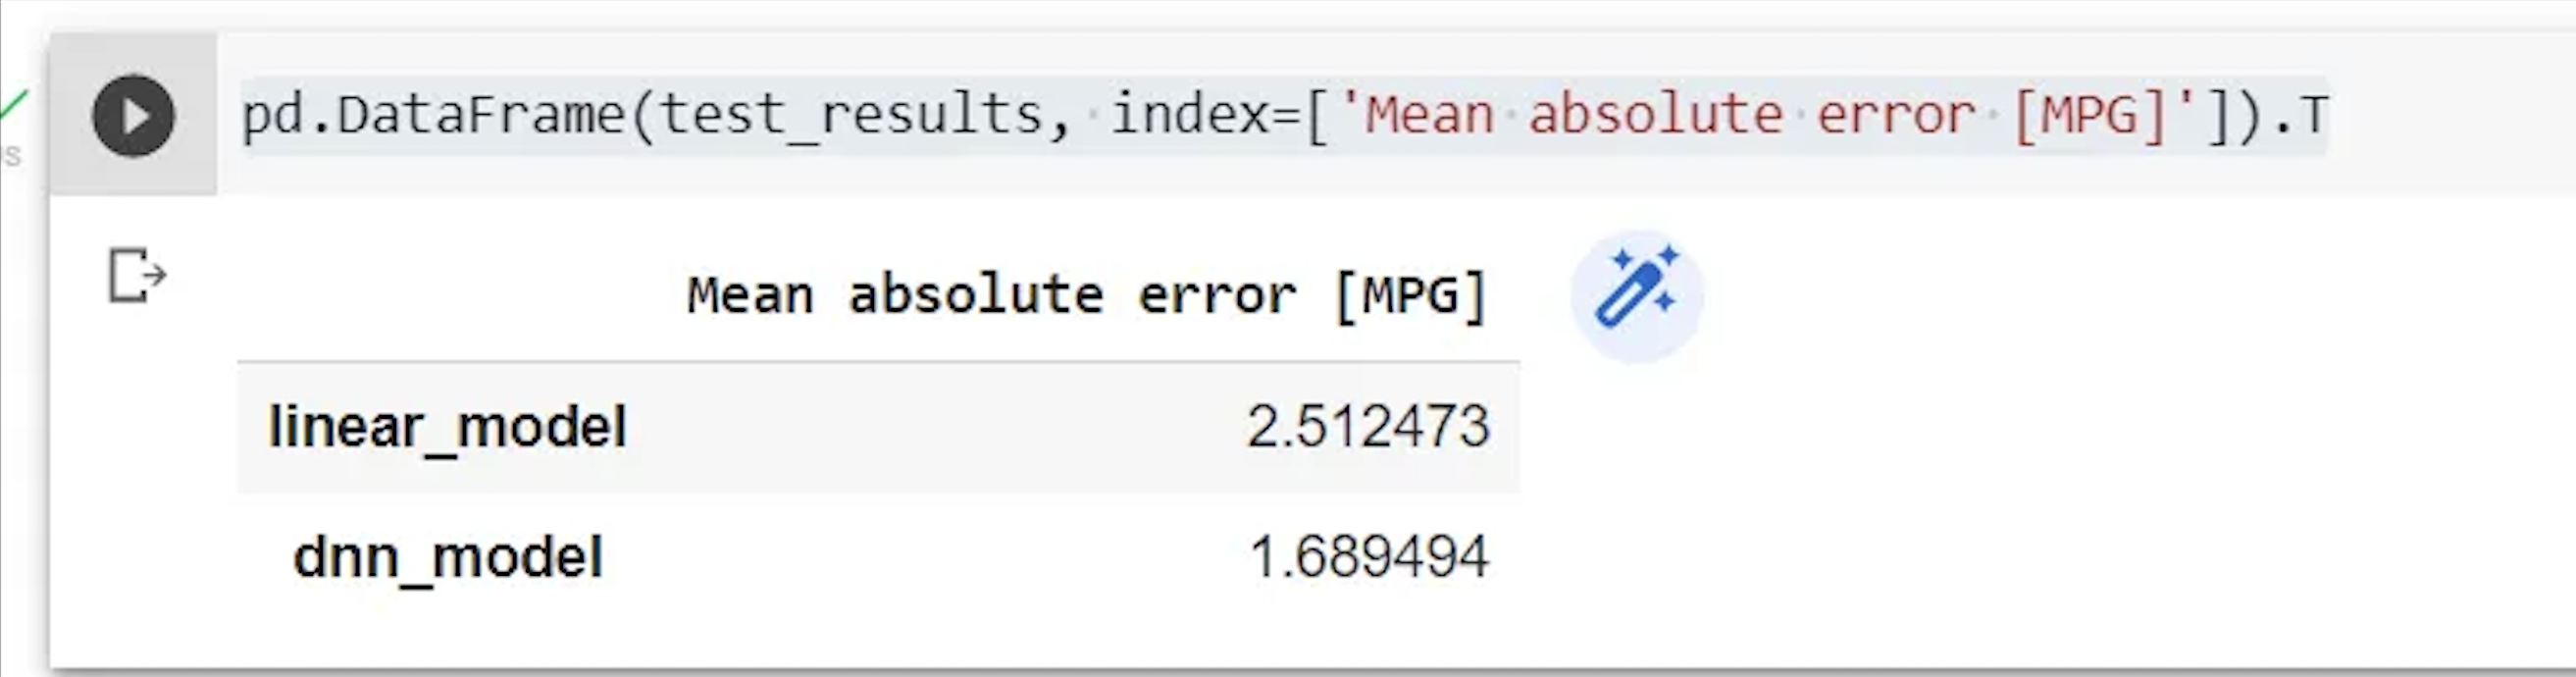
\includegraphics[scale=0.3]{Lineapy/Modelperformance.png}
		\caption{Model performance comparision}
		\label{fig:Model performance comparision}
	\end{figure}
	

	\textbf{in this case , the DNN model is better than the linear regression model. Hence we now save the DNN model.}
	
\begin{lstlisting}[language=Python]
	/**
	* @brief Saves a machine learning model as a LineaPy artifact.
	*
	* This function uses the LineaPy library to save a specified object 
	* (in this case, a deep neural network model) into the LineaPy artifact store.
	*
	* @param dnn_model The trained deep neural network model to be saved.
	* @param 'dnn_model' The name given to the artifact for future reference.
	* @return A LineaPy artifact object representing the saved model.
	*/
	model_artifact = lineapy.save(dnn_model, 'dnn_model')
\end{lstlisting}
	
	\pagebreak
	\textbf{To display the code of the model, use the get() method.}
	
	\begin{lstlisting}[language=Python]
		/**
		* @file model_training.py
		* @brief This script builds and trains a DNN model using TensorFlow.
		* 
		* This code was generated using LineaPy's get_code() method. It performs the 
		* following operations:
		* - Loads preprocessed training features and labels.
		* - Defines a deep neural network (DNN) model.
		* - Compiles and trains the model.
		* 
		* @note The script relies on pre-saved data stored as pickle files.
		*/
		
		import pickle
		import lineapy
		import tensorflow as tf
		from lineapy.utils.utils import prettify
		from tensorflow import keras
		from tensorflow.keras import layers
		
		/**
		* @brief Loads training features and labels from serialized pickle files.
		* 
		* @return train_features1 The preprocessed training features.
		* @return train_labels1 The corresponding training labels.
		*/
		normalizer = tf.keras.layers.Normalization(axis=-1)
		train_features1 = pickle.load(open("/root/.lineapy/linea_pickles/yzU2NLl", "rb"))
		train_labels1 = pickle.load(open("/root/.lineapy/linea_pickles/GPSupKi", "rb"))
		
		/**
		* @brief Builds and compiles a deep neural network model.
		* 
		* @param norm A TensorFlow normalization layer for preprocessing input data.
		* @return model A compiled Keras Sequential model.
		*/
		def build_and_compile_model(norm):
		model = keras.Sequential(
		[
		norm,
		layers.Dense(64, activation="relu"),
		layers.Dense(64, activation="relu"),
		layers.Dense(1),
		]
		)
		model.compile(loss="mean_absolute_error", optimizer=tf.keras.optimizers.Adam(0.001))
		return model
		
		/**
		* @brief Initializes the model and trains it with the provided data.
		* 
		* @note Training runs for 100 epochs with a validation split of 20%.
		* 
		* @param train_features1 Training features loaded from pickle.
		* @param train_labels1 Training labels loaded from pickle.
		*/
		dnn_model = build_and_compile_model(normalizer)
		history = dnn_model.fit(
		train_features1, train_labels1, validation_split=0.2, verbose=0, epochs=100
		)
	\end{lstlisting}
	

	\textbf{List all the saved artifacts.}
	
\begin{lstlisting}[language=Python]
	/**
	* @file lineapy_catalog.py
	* @brief Demonstrates the use of LineaPy to list all saved artifacts.
	* 
	* This script uses the LineaPy library to catalog all previously saved
	* artifacts in the current environment.
	* 
	* @author [Your Name]
	* @date [Insert Date]
	* @version 1.0
	* @see https://docs.lineapy.io for more details on LineaPy.
	*/
	
	/**
	* @function lineapy.catalog
	* @brief Lists all saved artifacts in LineaPy.
	* 
	* This function queries the LineaPy metadata database and returns a list
	* of all saved artifacts.
	* 
	* @return List of saved artifacts.
	*/
	lineapy.catalog()
\end{lstlisting}
	
	\pagebreak
	\textbf{The output-displays all the artifacts stored}

		\begin{figure}[h!]
		\centering
		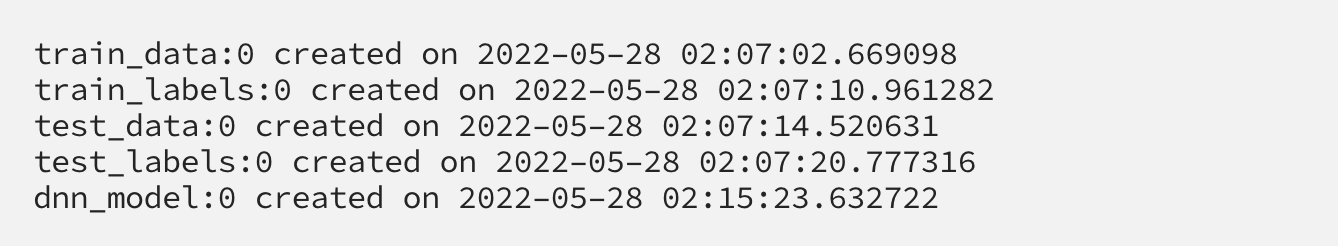
\includegraphics[scale=0.5]{Lineapy/Outputartifcats.png}
		\caption{Artifacts stored output}
		\label{fig:Artifacts stored output }
	\end{figure}
	

	\textbf{Now you can also build a data pipeline with the artifacts you have saved. The code to generate the pipeline are}
	
\begin{lstlisting}[language=Python]
	/**
	* @file example_code.py
	* @brief Example of using LineaPy to retrieve artifacts and prepare them for pipeline execution.
	* 
	* This script demonstrates how to retrieve artifacts stored in LineaPy using
	* their names and document their usage with Doxygen comments.
	*/
	
	/**
	* @brief Retrieve the training data artifact.
	* 
	* Fetches the artifact stored in LineaPy with the name "train_data"
	* and assigns it to a variable for further use.
	*/
	train_art = lineapy.get("train_data") ///< LineaPy artifact for training data
	train_art                            ///< Output: LineaArtifact(name='train_data', _version=0)
	
	/**
	* @brief Retrieve the training labels artifact.
	* 
	* Fetches the artifact stored in LineaPy with the name "train_labels"
	* and assigns it to a variable for further use.
	*/
	y_art = lineapy.get("train_labels")  ///< LineaPy artifact for training labels
	y_art                                ///< Output: LineaArtifact(name='train_labels', _version=0)
	
	/**
	* @brief Retrieve the trained DNN model artifact.
	* 
	* Fetches the artifact stored in LineaPy with the name "dnn_model"
	* and assigns it to a variable for further use.
	*/
	model_art = lineapy.get("dnn_model") ///< LineaPy artifact for trained DNN model
	model_art                            ///< Output: LineaArtifact(name='dnn_model', _version=0)
\end{lstlisting}
	
	\pagebreak
	\textbf{Now build the data pipeline.
	\begin{itemize}
		\item Pre-processed data.
		\item Model building
	\end{itemize}
	}
	
	\begin{lstlisting}[language=Python]
		/**
		* @brief Generate an Airflow pipeline using LineaPy
		*
		* This function creates an Airflow pipeline with specified artifacts and dependencies, 
		* and writes the pipeline files to the specified output directory.
		*
		* @param train_art.name The name of the training data artifact.
		* @param y_art.name The name of the target labels artifact.
		* @param model_art.name The name of the model artifact.
		* @param framework The workflow framework for the pipeline (default: "AIRFLOW").
		* @param pipeline_name The name of the pipeline to be generated.
		* @param dependencies A dictionary specifying dependencies between pipeline tasks.
		* @param output_dir The output directory for the pipeline files. Defaults to "AIRFLOW_HOME/dags".
		*
		* @return None
		*/
		directory = lineapy.to_pipeline(
		[train_art.name, y_art.name, model_art.name], 
		framework='AIRFLOW',
		pipeline_name="dnn_pipeline",
		dependencies={'dnn_pipeline_dnn_model': {'dnn_pipeline_train_data', 'dnn_pipeline_y'}},
		output_dir=os.environ.get("AIRFLOW_HOME", "~/airflow") + "/dags"
		)
	\end{lstlisting}
	
\textbf{	Final output files would look like this :}
	
	\begin{figure}[h!]
		\centering
		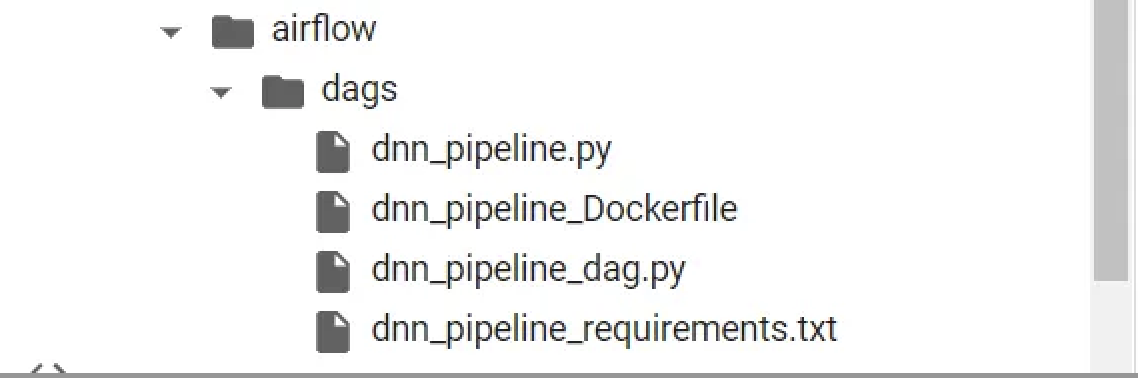
\includegraphics[scale=0.7]{Lineapy/Exampleoutputfiles.png}
		\caption{Output files}
		\label{fig:Output files }
	\end{figure}
	
	
	\pagebreak
	\begin{itemize}
		\item \textbf{Artifacts} is the list of artifact names to be used for the pipeline. Here we are using the train and model artifacts. Actually, we don’t need the test artifact.
	\item \textbf{pipelinename} is the name of the pipeline. 
	\item \textbf{dependencies} is the dependency graph among artifacts
	\item If artifact A depends on artifacts B and C, then the graph is specified as { A: { B, C } }
	\item If A depends on B and B depends on C, then the graph is specified as { A: { B }, B: { C } }

	\item \textbf{output\_dir} is the location to put the files for running the pipeline
	\item \textbf{framework} is the name of the orchestration framework to use
	\item LineaPy currently supports \textbf{"AIRFLOW"} and \textbf{"SCRIPT"}
	\item If \textbf{"AIRFLOW"}, it will generate files that can run Airflow DAGs. You can execute the file in airflow CLI.
	\item If \textbf{"SCRIPT"}, it will generate files that can run the pipeline as a Python script
\end{itemize}
	
	\section{LineaPy: Streamlining Data Science Workflows}
	
	LineaPy is a Python library that streamlines data science workflows by capturing, analyzing, and automating tasks involved in development. It traces code execution to comprehensively comprehend its context, enabling it to offer a range of tools facilitating swift transition to production for data scientists. With just two lines of code, LineaPy simplifies the process, aiding in quicker and easier deployment.
	
	\subsection{Facilitating Data Pipeline Development:}
	\begin{itemize}
		\item LineaPy expedites the transition from data science prototypes to operational data pipelines, enabling swift progression towards production-ready solutions.
		\item It facilitates the transformation of complex notebook code into structured and efficient data pipelines, ensuring smooth integration into orchestration systems.
		\item Through automated refactoring and code cleanup, LineaPy enhances code quality, reducing bugs and eliminating extraneous code, thereby accelerating the time to achieve valuable insights.
	\end{itemize}
	
	\subsection{Enhanced Understanding and Support:}
	\begin{itemize}
		\item LineaPy's core functionality involves analyzing the sequence of code execution to gain a thorough understanding of the code and its surrounding context.
		\item Leveraging this understanding, LineaPy furnishes a suite of robust tools designed to aid data scientists in seamlessly transitioning their work from experimentation to production environments.
	\end{itemize}
	
	\subsection{Key Functionalities:}
	\begin{itemize}
		\item \textbf{Modular Component Development}: Create adaptable and reusable components to construct flexible data pipelines.
		\item \textbf{Data Lineage Tracking}: Gain insights into the lineage of your data and associated artifacts to facilitate traceability and accountability.
		\item \textbf{Seamless Integration}: LineaPy seamlessly integrates with various Python libraries, preserving the continuity of existing workflows.
		\item \textbf{Automated Pipeline Generation}: Streamline pipeline development by automating the generation of pipelines across popular frameworks, eliminating redundant manual effort.
	\end{itemize}

	\section{Further Reading}
	
	To learn more about LineaPy, visit their \href{https://lineapy.org/}{official website} or their \href{https://github.com/LineaLabs/lineapy}{GitHub repository}.
	
	If you want to learn more about their use in MLops , with more detailed examples visit \href{https://towardsdatascience.com/lineapy-data-science-workflow-in-just-two-lines-mlops-made-easy-679f36ac63bd}{LineaPy Data Science Workflow In Just Two Lines: MLOps Made Easy} by Senthil E. 
\end{document}
